
\vspace{1cm}
\item A bola de \SI{0.5}{\kilogram} é disparada pelo dispositivo com mola mostrado. Determine a menor rigidez $k$ necessária para disparar a bola a uma distância máxima $s=\SI{750}{\milli\meter}$ plano acima após a mola ser empurrada para trás \SI{75}{\milli\meter} e a bola ser solta do repouso. Os quatro cabos $C$ e a placa $P$ mantêm a mola comprimida \SI{50}{\milli\meter} quando não há nenhuma carga sobre a placa.

\import{answers/}{answer-13}

\vspace{2cm}
\begin{flushright}
	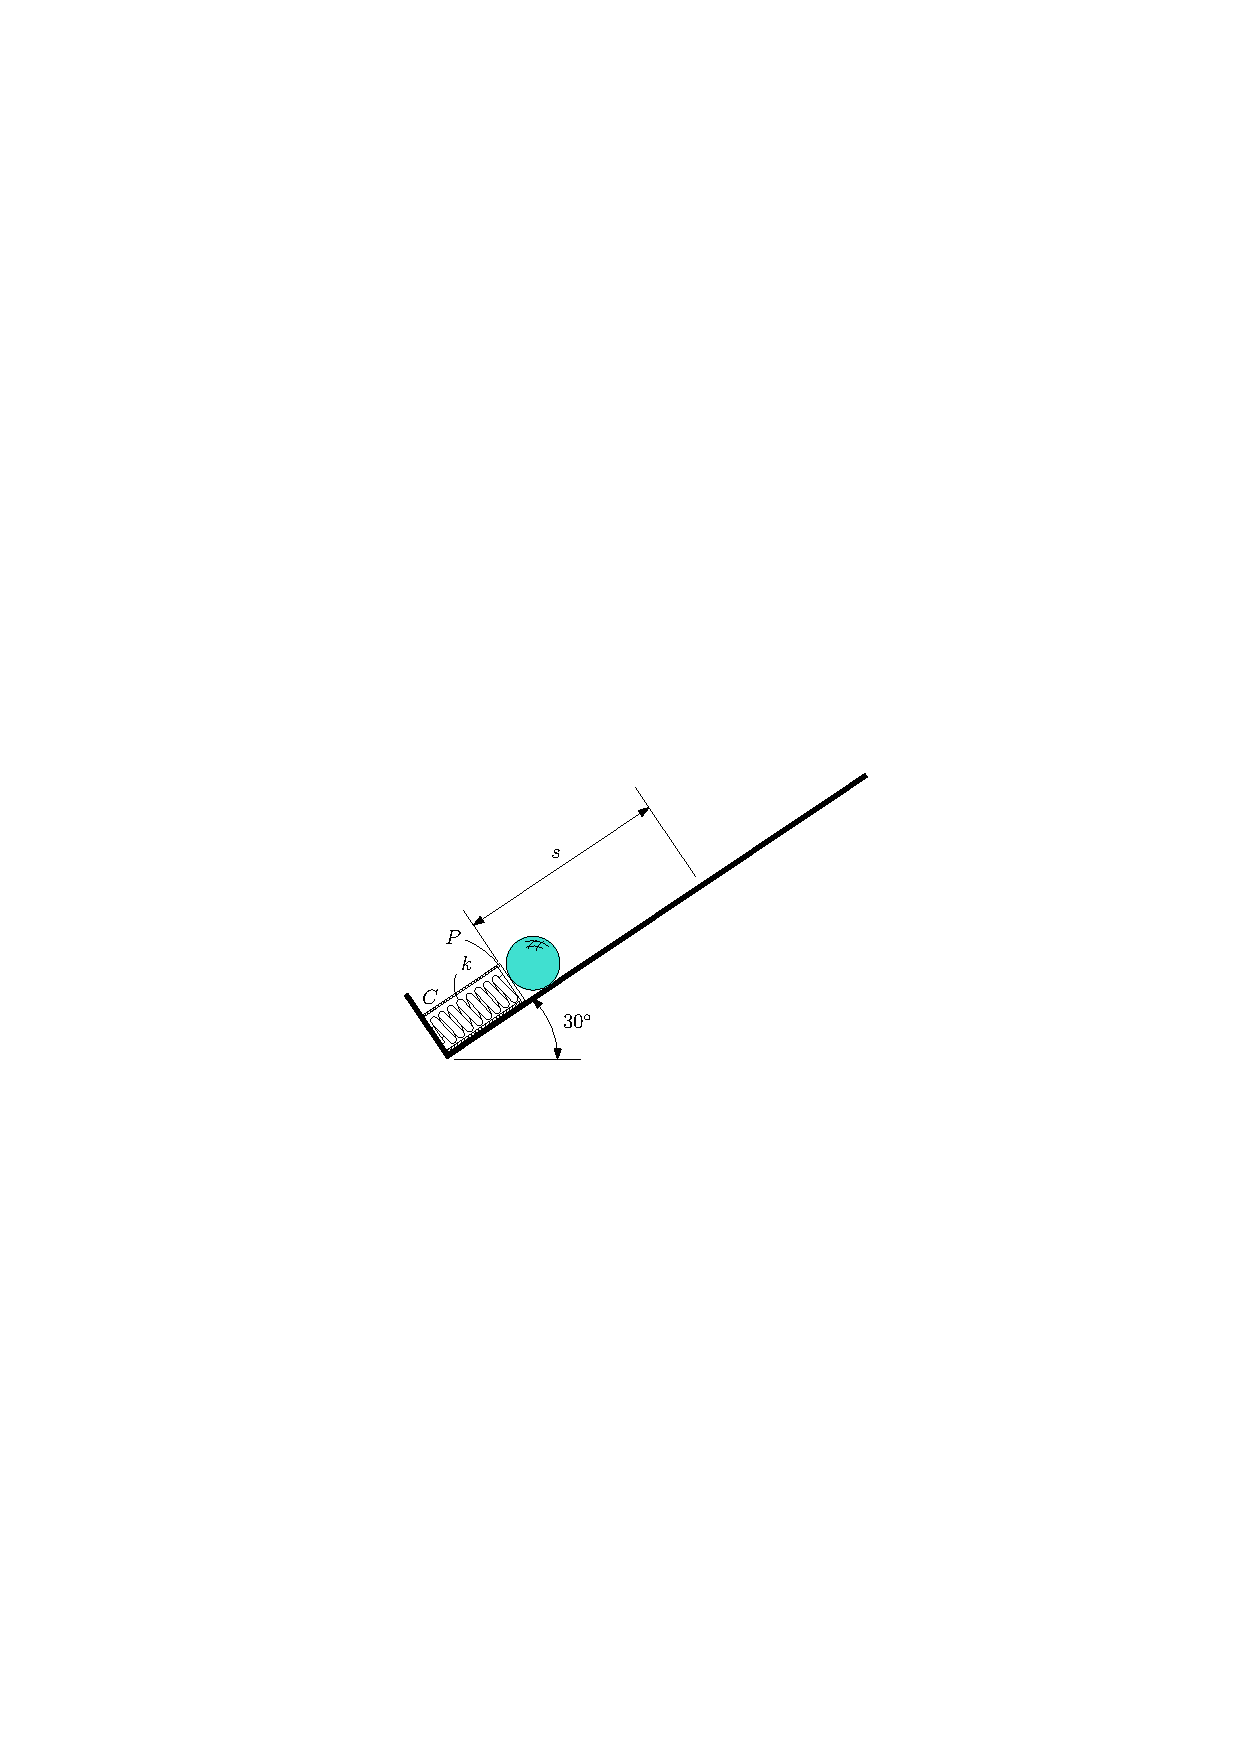
\includegraphics[scale=1.5]{images/draw_13.pdf}
\end{flushright}